\section{Megvalósítás}

Ebben a fejezetben részletesen bemutatásra kerül a rendszer megvalósítása, a projekt kezdeti létrehozásától kezdve a mappa- és fájlstruktúra leírásán át a legfontosabb funkciók implementációjáig. A cél egy átláthatóan felépített alkalmazás létrehozása, amely mind a felhasználói, mind az adminisztratív felületen stabil és könnyen karbantartható működést biztosít.

\subsection{A projekt létrehozása és környezet beállítása}

A fejlesztés Microsoft Visual Studio 2022 környezetben valósult meg, a .NET 8.0 keretrendszerre építve. A projekt típusa \textit{ASP.NET Core MVC Web Application}, amely a model-view-controller (MVC) architektúra elveit követi, lehetővé téve az üzleti logika, a megjelenítés és az adatkezelés hatékony rendszerezését.

Az adatkezeléshez az Entity Framework Core komponenst használtam, a Code First megközelítés segítségével. Az Entity Framework Core egy modern ORM technológia a .NET alkalmazások számára, amely lehetővé teszi az adatbázis-műveletek magas szintű megvalósítását. Ennek köszönhetően a modellosztályok a programkódban lettek definiálva, majd migrációk létrehozásával az adatbázis-struktúra automatikusan generálódott. Ez a módszer rugalmasságot biztosít a fejlesztés során, és egyszerűsíti az adatbázis módosítását.

Az alkalmazás egy SQL Server Express alapú relációs adatbázist használ, amely helyi környezetben gyors, megbízható és könnyen konfigurálható megoldást biztosít a fejlesztéshez. Az adatbázis kezelése teljesen az Entity Framework migrációs rendszerére épül.

\subsection{A megvalósítás mappastruktúrája és fő komponensei}

A projekt létrehozása a Visual Studio 2022 fejlesztőkörnyezet és a .NET 8 keretrendszer segítségével valósult meg. Az így generált mappastruktúra jól rendszerezett és könnyen bővíthető, támogatja az átlátható fejlesztést, és megkönnyíti az egyes komponensek logikai szétválasztását.

A \texttt{Controllers} mappa azokat az osztályokat tartalmazza, amelyek a felhasználói interakciókat kezelik és az adatokat feldolgozzák a működési logika szerint. Ezek a vezérlők külön-külön foglalkoznak az egyes entitásokkal, például a menetrendekkel, jegyekkel vagy felhasználókkal, biztosítva az adatok és a nézetek közötti kapcsolatot.

A \texttt{Models} könyvtár tartalmazza azokat az osztályokat, amelyek az adatbázisban tárolt entitásokat képezik, például a \texttt{Ticket}, \texttt{Contact} vagy \texttt{Schedule} osztályokat. Ezek az osztályok felelősek az adatok szerkezetének és az entitások közötti kapcsolatok megvalósításáért. Tulajdonképpen ezek az osztályok képezik az adatbázis tábláinak mintáját.


\subsection{Adatmodell és adatbázis felépítése}

Miután a projektet létrehoztuk, elsőként az alkalmazás alapját képező osztályokat, azaz a modelleket kellett létrehozni. Ezek az osztályok az adatbázisban tárolt adattáblákat írják le, és tartalmazzák a hozzájuk tartozó tulajdonságokat, valamint az egymással kialakított relációkat. Az előzetesen elkészített adatbázis-terv alapján hoztam létre a \texttt{AdminMessage}, \texttt{AdminTask}, \texttt{Attachment}, \texttt{Bus}, \texttt{Contact}, \texttt{RouteStop}, \texttt{Schedule}, \texttt{Stop}, \texttt{Ticket}, valamint \texttt{TransportRoute} osztályokat. Fontos kritérium volt, hogy az entitások közötti relációkat pontosan és figyelmesen implementáljuk. Itt az elsődleges kulcsok (Primary Key), illetve az idegen kulcsok (Foreign Key) helyes használatára kellett különös figyelmet fordítani.

A \texttt{Contact} osztályt az ASP.NET Identity komponens \texttt{IdentityUser} ősosztályából származtattam, amely beépített megoldást kínál a felhasználók szerepkörének zökkenőmentes implementálására és kezelésére.

A modellek és az adatbázis közötti kapcsolatot az \texttt{AppDbContext} osztály biztosítja, amely az Entity Framework Core egyik központi komponense. Ez az osztály az \texttt{IdentityDbContext} ősosztályból származik, és célja, hogy konfigurálja, kezelje és összekapcsolja a modelleket, sablonként szolgálva. Az \texttt{AppDbContext} osztályban találhatóak a \texttt{DbSet} típusú tulajdonságok, amelyek egy-egy tábla leképezését valósítják meg, például: \texttt{public DbSet Stops { get; set; }}, \texttt{public DbSet Schedules { get; set; }}.

Ezen felül az \texttt{AppDbContext} lehetőséget biztosít az entitások viselkedésének testreszabására az \texttt{OnModelCreating} metódusban, ahol külön definiálhatjuk a kulcsokat, kapcsolatokat, korlátozásokat, valamint egyéb konfigurációkat. Különösen hasznos az úgynevezett "vízesés törlés" (cascade delete) viselkedés figyelembe vétele, amely során egy entitás törlése vízesésszerűen magával vonhatja más kapcsolódó entitások törlését is. Az \texttt{OnModelCreating} metódus lehetőséget biztosít ennek felügyelésére, ezáltal elkerülve az adatvesztést okozó nem kívánt láncfolyamatokat.

\begin{figure}[H]
\centering
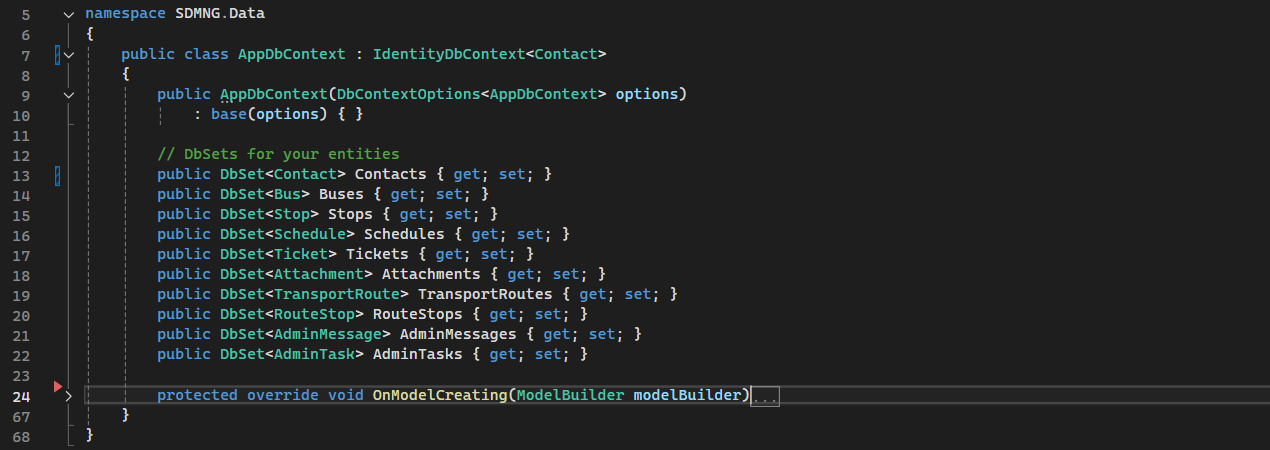
\includegraphics[width=1\textwidth]{Szakdolgozat/Mellekletek/AppDbContext.PNG}
\caption{A projektem AppDbContext osztálya látható az általam definiált modellekkel kiegészítve. }
\label{fig:appdbcontext}
\end{figure}

A \ref{fig:appdbcontext}. ábrán látható, a rendszeremben létrehozott osztályok segítségével létrehozott struktúra, amely a helyes adatbázis megvalósításában játszik kulcsszerepet. Az AppDbContext nevű osztályt az IdentityDbContext ősosztályból származtattam, majd egészítettem ki.
\vspace{\baselineskip}


Az AppDbContext osztály beállítása után szükség volt az adatbázis-fájl konfigurálására. A projekt \texttt{appsettings.json} fájlban megadtuk az adatbázis elérési útvonalát a \texttt{ConnectionStrings} szekcióban.

\begin{figure}[H]
\centering
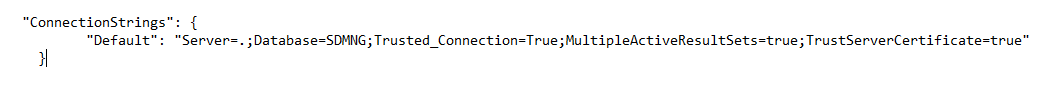
\includegraphics[width=1\textwidth]{Szakdolgozat/Mellekletek/Connectionstring.PNG}
\caption{Az adatbázis kapcsolódási kulcsa a lokális adatbázishoz.}
\label{fig:connectionstring}
\end{figure}

A \ref{fig:connectionstring}. ábrán a projektben használt \textit{connection string} látható, amely a lokális SQL Server adatbázishoz való kapcsolódást valósítja meg. Ez tartalmazza az SDMNG adatbázis elérési útvonalát, az adatbázis nevét, valamint a hitelesítési mód beállításait.
\vspace{\baselineskip}

Miután a konfigurációs fájlokat megfelelően implementáltuk, és a modellosztályaink is a tervek szerint készültek el, elérkezett az idő az első migráció létrehozására. Az adatbázis felépítését az Entity Framework migrációs rendszerével valósítottam meg. Az első migráció elkészítéséhez a terminálban a következő parancsot használtuk: 
\begin{lstlisting}
dotnet ef migrations add CreateDatabase
\end{lstlisting}
A parancs végrehajtása után a Migrations mappában létrejött a fentebb megadott névvel rendelkező migrációs fájl. Ezen a ponton fontos még egyszer ellenőrizni a generált adatbázis-entitásokat, és különös hangsúlyt kell fektetni a relációk helyességére. Amennyiben minden a terv szerint valósult meg, végrehajtjuk az adatbázis fizikai létrehozására vagy frissítésére szolgáló parancsot: 
\begin{lstlisting}
dotnet ef database update
\end{lstlisting}

Ez a parancs a korábban generált migrációs fájlok alapján felépíti vagy kiegészíti az adatbázist a megadott kapcsolati karakterlánc (connection string) segítségével.

\subsection{Vezérlők (Controllers) felépítése és működése}
Az alkalmazás működésének egyik kulcseleme a vezérlők rendszere. Ezek azok az osztályok, amelyek közvetlen kapcsolatban állnak a felhasználóval: fogadják az oldalkéréseket, előkészítik az adatokat, és eldöntik, milyen nézetet kell megjeleníteni vagy milyen műveletet kell végrehajtani. A vezérlők az MVC architektúra "C" komponensét képviselik, tehát az alkalmazás logikai magját képezik.

A projektben minden jelentősebb funkció – például jegyvásárlás, menetrendkezelés, felhasználói adatok kezelése – külön vezérlőt kapott. Ezek az osztályok a \texttt{Controllers} nevű mappában találhatóak, és  a \texttt{Controller} alaposztályból öröklődnek.

\subsubsection{A konstruktor szerepe}
A vezérlők konstruktorában történik meg az úgynevezett függőséginjektálás (dependency injection). Ez azt jelenti, hogy a vezérlő induláskor automatikusan megkapja azokat a szolgáltatásokat vagy komponenseket, amelyekre működése során szüksége lesz – például az adatbázis-kapcsolatot biztosító \texttt{AppDbContext} példányt.

\subsubsection{Aszinkron metódusok (async/await)}
A vezérlők fejlesztése során aszinkron metódusok használtam. Ennek elsődleges oka, hogy ezek a módszerek hatékonyabb működést tesznek lehetővé, különösen akkor, amikor a rendszer külső erőforráshoz – például adatbázishoz – fordul adatlekérés vagy módosítás céljából. Ilyen esetekben a programnak várnia kell a válaszra, és ha ez a várakozás egy szinkron módon írt metódusban történik, az idő alatt az egész kérés „lefagyhat”, nem képes más feladatokra reagálni.

Az aszinkron működés lényege, hogy ezek a metódusok nem akadályozzák az alkalmazás többi részének futását, miközben például háttérben adatokat kérnek le vagy dolgoznak fel. Ez különösen fontos egy webalkalmazás esetén, ahol egyszerre több felhasználói kérés is érkezhet – például jegyvásárlás, menetrend megtekintés vagy felhasználói adatok kezelése. Az \texttt{async/await} kulcsszavak használatával ezek a műveletek párhuzamosan, egymást nem akadályozva tudnak végbemenni.

Az aszinkron működés megvalósításában kulcsszerepet játszik két kifejezés: az \texttt{async} és az \texttt{await}. Az \texttt{async} kulcsszóval azt jelezzük a rendszernek, hogy az adott metódus tartalmazhat olyan műveleteket, amelyek végrehajtása hosszabb időt vesz igénybe, és ezeket érdemes nem blokkoló módon kezelni. Ezzel előkészítjük a metódust arra, hogy akár több lépésben, megszakítható módon fusson le.

Az \texttt{await} pedig azt mondja a programnak: itt most egy időigényes művelet következik – például adatbázis-lekérdezés vagy fájl beolvasása –, és a vezérlés addig adódjon vissza a hívó félnek, amíg ez be nem fejeződik. A lényeg az, hogy a várakozás ideje alatt a többi feladat nem áll meg, az alkalmazás közben más kéréseket is képes kiszolgálni.

Egy-egy metódus így nemcsak hatékonyabb, de a felhasználói élményt is képes pozitívan befolyásolni, mivel csökken a válaszidő, gyorsabban jelennek meg az oldalak, és kevesebb az esély a hibákra vagy „megakadásokra”. A projekt során ezért az adatbázissal kapcsolatos lekérdezések és módosítások szinte minden esetben aszinkron módon lettek megvalósítva.

\subsubsection{Hibakeresés, csatolmánykezelés}
Az alkalmazás készítése közben nagyon fontos szerepet kapott a naplózás és a környezeti beállítások kezelése, mert ezek segítenek gyorsan megtalálni a hibákat és biztosítják, hogy a rendszer megbízhatóan működjön. A fejlesztés során az ASP.NET Core beépített \texttt{ILogger} felületét használtam, ami egy hatékony eszköz a különféle események naplózására. Ez azt jelenti, hogy az alkalmazás működésével kapcsolatos fontos információkat — például figyelmeztetéseket vagy hibákat — eltárolhatjuk, így könnyebben nyomon követhető, mi történik a háttérben, és gyorsan rá lehet jönni, ha valami nem működik jól.

Az \texttt{ILogger} segítségével például a fájlok feltöltésekor vagy e-mail küldéskor felmerülő hibák részletesen naplózhatóak, így visszakövethetővé válik, hogy mikor és milyen körülmények között jelentkezett az adott hiba. Ez különösen hasznos fejlesztési és tesztelési fázisban, amikor az alkalmazás viselkedését pontosan felügyelni kell.

A csatolmányok feltöltésekor az \texttt{IWebHostEnvironment} segítségével meghatároztam a fájlok fizikai tárolási helyét, amely általában a \texttt{wwwroot/} mappában található. Ez a megközelítés lehetővé teszi, hogy a különböző környezetekben eltérő útvonalakat használjunk, megkönnyítve ezzel a fejlesztést és a telepítést. A feltöltött fájlok elérését pedig dinamikusan, az alkalmazás futási környezetétől függően kezeljük.

\subsubsection{Biztonság és hitelesítés a vezérlők szintjén}
A vezérlők kialakításakor különös figyelmet fordítottam a biztonsági elvekre. Az ASP.NET Identity keretrendszer biztosította a hitelesítés és szerepkör-alapú jogosultságkezelés infrastruktúráját. Az alkalmazásban minden vezérlő és metódus, amely érzékeny adatot kezel vagy kizárólag regisztrált felhasználók számára elérhető, az \texttt{[Authorize]} attribútummal van ellátva. Egyes metódusoknál szerepkörhöz kötött elérés is alkalmazásra került, például az adminisztrációs felületek esetében kizárólag az Admin szerepkörrel rendelkező felhasználók végezhetnek műveleteket.

A \texttt{[Authorize]} attribútum legfontosabb megjelenési formája a bejelentkezés utáni jogosultság-kezelés: amennyiben a felhasználó nem azonosította magát, vagy nem rendelkezik a megfelelő szerepkörrel, nem férhet hozzá bizonyos oldalakhoz és műveletekhez. Ezáltal biztosítható, hogy például az adminisztrátor által elérhető listázási, szerkesztési vagy törlési funkciókat egy egyszerű, be nem jelentkezett felhasználó ne láthassa vagy használhassa.

A jelszavak kezelése az ASP.NET Identity rendszer beépített funkcióin keresztül történik, amely a felhasználói jelszavakat biztonságos módon, hashing algoritmus alkalmazásával tárolja az adatbázisban. A jelszavak visszafejtése nem lehetséges, csak a hash-értékek kerülnek mentésre. Ez alapértelmezett védelem a jogosulatlan hozzáférés ellen, még akkor is, ha valaki illetéktelenül hozzájutna az adatbázishoz.

\subsection{Fontosabb kontrollermetódusok megvalósítása}
\subsubsection{JegyController metódusok (Ticket)}
A fejlesztés során több olyan vezérlőmetódus készült, amelyek összetettebb funkciókat látnak el, például a jegyvásárlási folyamat kezelését. Ez magában foglalja a vásárlás rögzítését, a QR-kód generálását, valamint a felhasználó számára történő visszaigazolást e-mail formájában.

A jegyvásárlási folyamat egyik fontos lépése a QR-kód generálása, amely egy útvonalat tárol, pontosabban egy URL-t tartalmaz, amely a webalkalmazás adott oldalára — például a jegy részleteit bemutató Ticket Detail oldalra — mutat. Ez az URL tartalmazza a jegy egyedi azonosítóját, így a QR-kód beolvasásakor a felhasználó közvetlenül a megfelelő oldalra jut. A QR-kód generálása általában egy erre alkalmas, külső könyvtár vagy csomag segítségével történik, amely az URL-t vizuális, képi formátumba alakítja át (például PNG formátumú képpé), és ezt a képet az alkalmazás vagy az e-mail csatolmányaként használja fel.

Az e-mail küldése során az SMTP (Simple Mail Transfer Protocol) protokollt használjuk, amely egy széles körben elterjedt, szabványos megoldás az elektronikus levelek továbbítására. A folyamat során beállítjuk az SMTP szerver adatait, mint például a hosztnevet (pl. smtp.gmail.com), a portszámot, valamint a biztonsági protokollt (SSL vagy TLS). A hitelesítéshez szükséges a felhasználónév és az alkalmazás-specifikus jelszó, különösen ha a Gmail kétlépcsős azonosítását használjuk, mivel ilyenkor a normál jelszó nem használható az SMTP klienshez. Az e-mail összeállítása tartalmazza a címzett, a tárgy, és a levél törzsének megadását, amely akár HTML formátumban is megjelenhet, így lehetőség nyílik például a QR-kód beágyazására vagy mellékletként való csatolására. A levél elküldése aszinkron módon történik, hogy ne akadályozza a webalkalmazás egyéb működését.

A Google-fiókok biztonságos használatához ajánlott a kétfaktoros hitelesítés (2FA) beállítása, amely a jelszó mellett egy további, egyszer használatos kód megadását követeli meg. Ez a kód általában egy mobilalkalmazással, például a Google Authenticatorral generált, időalapú számsorozat, vagy SMS-ben érkező üzenet formájában érkezik. Ha 2FA engedélyezve van, az SMTP szolgáltatásokhoz nem használható a fő jelszó, ezért alkalmazás-specifikus jelszót kell létrehozni a Google fiók biztonsági beállításaiban. Ez a jelszó kizárólag az adott program vagy szolgáltatás számára érvényes, és lehetővé teszi, hogy a rendszer biztonságosan csatlakozzon az SMTP szerverhez anélkül, hogy veszélyeztetné a fiók fő jelszavát.

Ahhoz, hogy a rendszer automatikusan vissza tudjon igazolni egy sikeres jegyvásárlást e-mailben — például egy QR-kódot tartalmazó üzenet formájában — elengedhetetlen, hogy megfelelő módon előkészítsük az SMTP-alapú levélküldés technikai hátterét.

A megvalósítás egyik alapköve az, hogy az érzékeny adatokat (például az e-mail címhez tartozó hitelesítési adatokat, a kiszolgáló nevét és portját) ne kódoljuk bele az alkalmazásba, hanem külső konfigurációs fájlba konfiguráljuk, például az appsettings.json állományba. Ez nemcsak tisztább kódot eredményez, de biztonsági és karbantarthatósági szempontból is előnyös.

A következő blokk egy példát mutat arra, hogyan nézhet ki ez a konfigurációs szekció az appsettings.json fájlban:

\subsubsection{Kapcsolatfelvétel a ContactController segítségével}

A kapcsolattartási funkció célja, hogy a felhasználók egyszerűen és gyorsan elérhessék az adminisztrátort, például kérdés, visszajelzés vagy technikai probléma esetén. Ennek megvalósításához egy űrlap áll rendelkezésre, ahol a látogató megadhatja nevét, e-mail címét, a téma tárgyát, valamint a saját üzenetét.

Az üzenet elküldése a háttérben e-mail formájában történik, az SMTP protokoll használatával. Mivel ezt a technikai megoldást korábban már részletesen bemutattam a JegyController működésénél, ahol a visszaigazolás és QR-kód küldés történt, itt csupán annak alapjaira hivatkozom. A konfigurációs részletek — például a kiszolgáló címe, portszám, hitelesítési mód, valamint az alkalmazásjelszavak és kétfaktoros azonosítás — megegyeznek az ott leírtakkal.

A különbség mindössze az üzenet tartalmában és a címzettben rejlik: míg a jegyvásárlás során egy automatikusan generált, HTML-alapú visszaigazolást küldünk ki, itt a felhasználó által kézzel írt üzenetet juttatjuk el az adminisztrátor előre meghatározott e-mail címére. Az e-mail továbbítása aszinkron módon történik, hogy ne akassza meg az alkalmazás működését.


\subsubsection{CRUD műveletek egységes megvalósítása a vezérlőkben}

A fejlesztés során az alkalmazás alapját az úgynevezett CRUD műveletek (Create, Read, Update, Delete) képezik, amelyek minden egyes entitás — legyen szó felhasználóról, jegyről, buszjáratról vagy akár kapcsolatfelvételről — kezelésének alapjai. Ezeket a funkciókat minden vezérlő (controller) esetében egységes logika mentén valósítottam meg, hogy átlátható és könnyen karbantartható struktúrát alakítsak ki.

\paragraph{Létrehozás (Create):}
Ez a művelet lehetővé teszi új adatok felvitelét az adatbázisba. Ez a funkció egy űrlap beküldésével történik, amelyet a frontendről kapott modell alapján dolgoz fel a controller. A POST típusú HTTP kérés során a kapott adatok validálás után bekerülnek az adatbázisba a kontextus objektum Add() vagy AddAsync() metódusával. A legtöbb vezérlőnél — például TicketController, BusController, ContactController — hasonló módon történik ez a feldolgozás.

\paragraph{Lekérdezés (Read):}
A meglévő adatok megjelenítése történik ezzel a művelettel. Itt főként GET típusú kérésekkel dolgozunk, amelyek során az adatbázisból ToListAsync(), FindAsync(), vagy FirstOrDefaultAsync() metódusokkal kérdezzük le az aktuális adatokat. Ezek az információk például a felhasználó által megvásárolt jegyek, vagy a rendszerben tárolt üzenetek részleteinek megtekintését szolgálják.

\paragraph{Módosítás (Update):}
Az adatok frissítésére a POST metódus szolgál, általában két lépésben. Először lekérdezzük a módosítani kívánt elemet (például egy meglévő busz útvonalát vagy egy kapcsolatfelvétel állapotát), majd az új adatokkal felülírjuk az eredetit, és végül a context.Update(entity) metódus segítségével mentjük el a módosított rekordot.

\paragraph{Törlés (Delete):}
A törléshez szükség van az adott entitás egyedi azonosítójára. Ezt általában GET vagy POST metódussal kapjuk meg a kliensoldalról. A lekérdezett objektumot ezután eltávolítjuk az adatbázisból a Remove() vagy RemoveRange() metódus segítségével. A TicketController például ezt használja jegyek törléséhez, míg a ContactController a beérkezett üzenetek kezelésénél.

\paragraph{Egységesítés előnyei:}
Azáltal, hogy minden controllerben hasonló logikát követtem a CRUD műveletek megvalósításánál, az alkalmazás könnyebben bővíthetővé és tesztelhetővé vált. A fejlesztés során a DbContext központosítása, valamint az aszinkron metódusok \texttt{await \_context.SaveChangesAsync()} következetes használata biztosította a gyors és megbízható adatkezelést.

\subsection{Nézetek (View) felépítése}

Az alkalmazásban a felhasználói felület megjelenítéséért az ASP.NET Core MVC nézetek (Views) felelősek, amelyek a vezérlők (Controller) által feldolgozott adatokat jelenítik meg. A nézetek szerepe, hogy az adatokat érthető és esztétikus formában mutassák be a felhasználóknak, miközben biztosítják a felhasználói interakció lehetőségét is.

A nézetek elsősorban Razor-szintaxissal készültek, amely egy egyszerű, de rugalmas eszköz az HTML és a C\# kód együttes kezelésére. Ez lehetővé teszi, hogy dinamikusan generáljuk az oldal tartalmát az adatbázisból érkező adatok alapján, miközben megőrizzük a tiszta és átlátható kódot.

A CRUD (Create, Read, Update, Delete) műveletek megvalósításához külön nézetek állnak rendelkezésre, amelyek mindegyike a megfelelő funkciót támogatja. Például a „Create” nézetben űrlapokat helyezünk el az új adatok beviteléhez, míg az „Index” vagy „List” nézet az adatbázisból lekérdezett elemek listáját jeleníti meg. A „Details” nézet egy adott elem részletes adatait mutatja be, az „Edit” pedig a módosításra szolgáló felületet biztosítja. Végül a „Delete” nézet megerősítő üzenetet jelenít meg a törlési művelet előtt.

A nézetdizájn során figyelmet fordítottam az átláthatóságra és a felhasználóbarát megjelenésre. Az alkalmazásban Bootstrap keretrendszert használtam, amely egy széles körben elterjedt CSS és JavaScript alapú eszköztár a reszponzív, modern weboldalak készítéséhez. A Bootstrap komponensek — például űrlapok, gombok, navigációs sávok és modális ablakok — segítségével egységes, könnyen kezelhető felületet sikerült kialakítani.

Az alkalmazás nézeteiben újrahasznosítható elemet alkalmaztam, mint például résznézeteket (Partial Views) és ViewComponent-eket. Ezek a komponensek lehetővé teszik, hogy az ismétlődő felhasználói felület részeket egyszer készítsük el, majd több helyen használjuk fel, ami jelentősen megkönnyíti a kód karbantartását és átláthatóságát. Különösen a felhasználói hitelesítéshez kapcsolódó oldalak, mint a bejelentkezés és regisztráció, a .NET Identity keretrendszer szolgáltatásaira épülnek. Ezeknél a funkcióknál résznézeteket használtam a vizuális elemek szervezésére, így egységes megjelenést és egyszerűbb kezelhetőséget biztosítva az autentikációs folyamatokhoz.

\subsection{Főbb Nézetek}
\subsubsection{Navigációs sáv és legördülő menü }
Az alkalmazás főbb vizuális elemei közé tartozik a navigációs sáv, amely a felhasználók számára elérhető oldalakat sorolja fel, mint például az állomások (Stations), útvonalak (Routes), saját jegyek (MyTickets), menetrendek (Schedule) és az elérhetőségek (Contact Me). 

Ezen felül a navigáció része egy olyan legördülő menü is, amely kizárólag az adminisztrátorok számára látható, az ő szerepkörükhöz igazodva. Ebben a menüben olyan adminisztratív oldalak találhatók, mint a teendők listája (ToDo List), csatolmányok (Attachments), megállók (Stops), buszok (Buses), útvonalak (Routes), menetrendek (Schedules), felhaszálók (Contacts) és jogosultságok (Roles). Minden egyes menüpont egy olyan listanézetre vezet, ahol az adminisztrátor az adott entitás összes adatát áttekintheti és kezelheti, mivel teljes körű jogosultságokkal rendelkezik.

\begin{figure}[H]
\centering
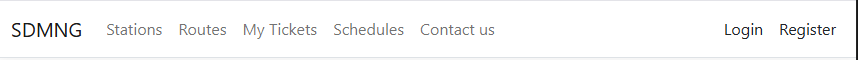
\includegraphics[width=1\textwidth]{Szakdolgozat/Mellekletek/navsavlogin0.PNG}
\caption{A navigációs sáv megjelenése bejelentkezés nélküli állapotban.}
\label{fig:navsav}
\end{figure}

A \ref{fig:navsav}. ábra a webalkalmazás fő navigációs sávját mutatja be abban az esetben, amikor a felhasználó még nem jelentkezett be. Ilyenkor a látogató kizárólag a nyilvános funkciókat érheti el, például a menetrendek, megállók vagy kapcsolatfelvételi űrlap megtekintését. A felső menüsor jobb szélén megjelennek a bejelentkezés „Login” és Regisztráció „Register” gombok, amelyek lehetőséget biztosítanak az azonosításra vagy új fiók létrehozására. Ebben az állapotban az adminisztrációs és egyéb jogosultsághoz kötött elemek nem láthatók, biztosítva ezzel a rendszer biztonságos és szerepkör-alapú elérhetőségét.


\begin{figure}[H]
\centering
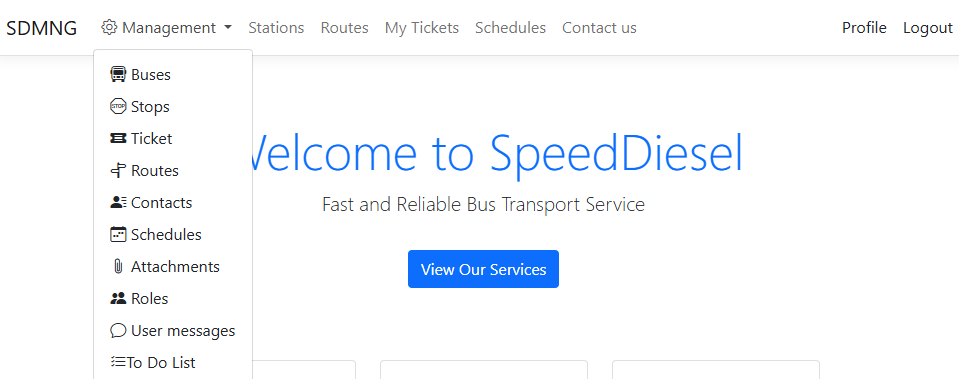
\includegraphics[width=1\textwidth]{Szakdolgozat/Mellekletek/navsavlogin1.PNG}
\caption{A navigációs sáv megjelenése bejelentkezett adminisztrátor számára.}
\label{fig:navsavlogged}
\end{figure}

A \ref{fig:navsavlogged}. ábrán a navigációs sáv bejelentkezett állapotban látható, adminisztrátori jogosultság mellett. Ebben az esetben a felhasználó számára elérhetővé válik egy további, legördülő menü, amely az adminisztrációs funkciókat csoportosítja. A menü tartalmazza többek között a megállók (Stops), buszok (Buses), útvonalak (Routes), menetrendek (Schedules), csatolmányok (Attachments), felhasználók (Contacts), jogosultságok (Roles), valamint teendők (ToDo List) kezelésére szolgáló linkeket. Ezek a nézetek csak az adminisztrátor szerepkörrel rendelkező felhasználók számára jelennek meg, és lehetőséget biztosítanak az alkalmazás teljes körű adatkezelésére és adminisztrálására. A menüsáv jobb oldalán továbbra is elérhető a kijelentkezési lehetőség, amely biztosítja a munkamenet megfelelő lezárását.


\vspace{\baselineskip}
\subsubsection{Lista oldalak}
A listanézetek felépítése egységes, ahol az adott entitáshoz tartozó legfontosabb adatokat oszlopokban mutatjuk be. Minden ilyen nézet tartalmaz egy „Actions” nevű oszlopot is, amelyben három alapvető művelet található: a részletek megtekintése (Detail), az adat módosítása (Modify/Edit), valamint az elem törlése (Delete). Ezek a gombok minden egyes listaelem mellett megjelennek, és mindegyikhez az adott elem egyedi azonosítója (ID) van hozzárendelve. Ennek köszönhetően, amikor egy felhasználó rákattint valamelyik művelet gombra, a sornak vagy elemnek megfelelő oldalt nyitja meg, így biztosítva a pontos és gyors navigációt az funkciókat megvalósító oldalak között.

Azokon az oldalakon, ahol az adatbevitel nem automatikusan történik — mint például a jegyek vagy az admin üzenetek — rendelkezésre áll egy „Create” gomb, amely új bejegyzések létrehozását teszi lehetővé. Érdemes megemlíteni, hogy a jegyek esetében a listaelemek nem közvetlenül itt jönnek létre, hanem a jegyvásárlási folyamat során, amikor a „Buy Ticket” funkció generál egy új rekordot az adatbázisba, amely aztán automatikusan megjelenik a jegyek listájában. Hasonló módon a „Contact Me” oldalon a felhasználó által elküldött üzenet szintén mentésre kerül az adatbázisba, és ezáltal megjelenik az adminisztrátorok számára készült üzenetlistában.

Minden oldal továbbá tartalmaz egy „Back” gombot, ami megkönnyíti a felhasználók számára a gördülékeny visszalépést az előző nézetekhez, ezzel is támogatva az intuitív és zökkenőmentes navigációt az alkalmazásban.

